% Group-meeting note: figure-first eight-page version.
% The formal manuscript is maintained separately in paper/formal/.
\documentclass[11pt]{article}
\usepackage[margin=2.2cm]{geometry}
\usepackage{amsmath,amssymb}
\usepackage{booktabs,array,tabularx}
\usepackage{tikz}
\usetikzlibrary{arrows.meta,positioning,calc}
\usepackage{pgfplots}
\usepgfplotslibrary{groupplots}
\pgfplotsset{compat=1.18}
\usepackage{float,enumitem,multicol,microtype}
\usepackage[round]{natbib}
\usepackage[font=small,skip=3pt]{caption}
\usepackage{titlesec}
\titlespacing*{\section}{0pt}{9pt plus 2pt}{4pt}
\titlespacing*{\subsection}{0pt}{7pt plus 2pt}{3pt}
\titlespacing*{\paragraph}{0pt}{5pt plus 1pt}{6pt}
\setlength{\abovedisplayskip}{4pt}
\setlength{\belowdisplayskip}{4pt}
\setlength{\abovedisplayshortskip}{2pt}
\setlength{\belowdisplayshortskip}{2pt}
\setlist[itemize]{leftmargin=*,topsep=2pt,itemsep=1pt,parsep=0pt}
\setlist[enumerate]{leftmargin=*,topsep=2pt,itemsep=2pt,parsep=0pt}
\newcolumntype{L}[1]{>{\raggedright\arraybackslash}p{#1}}
\newcommand{\ch}{\widehat c}
\newcommand{\E}{\mathbb E}
\newcommand{\regionkey}[2]{%
  \tikz[baseline=-0.45ex]{\draw[fill=#1,draw=black,line width=.25pt]
  (0,0) rectangle (.24,.15);}\,#2}

\begin{document}

\begin{center}
{\Large\bfseries Announced Rescue Pricing with Latent Market Thickness}\par
\vspace{2pt}
{\normalsize Group-meeting note --- benchmark, numerical pattern, and formal model}\par
\vspace{2pt}
{\small 27 August 2026}
\end{center}
\vspace{-5pt}

\noindent\textbf{Preview.}
A publicly known single driver gives an exact cutoff-WPBE and a closed-form
optimal menu.  With latent Poisson supply, the completion value of rescue
pricing is small in thin markets, largest at an intermediate thickness, and
small again in thick markets.  For
$(\alpha,\beta,\delta,\gamma)=(1,.8,.8,0)$, the deterministic numerical
solution peaks near $m=9.72$ and improves optimized completion by $6.16$
percentage points.  The endpoint pattern is proved; strict single-peakedness
is a conjecture.

\section{Exact one-rider/one-driver benchmark}

\subsection{Closed-form solution}

The rider has $v\sim U[0,1]$, the driver has $c\sim U[0,1]$, and the platform
maximizes completion.  Delayed rider value is $\beta v$ and delayed incumbent
surplus is $\delta(p_j-c)$.  The platform commits to
$0\le p_1\le p_2\le1$.  The number of drivers is publicly known to be exactly
one; there is no survival shock or fresh entry.

\begin{figure}[H]
\centering
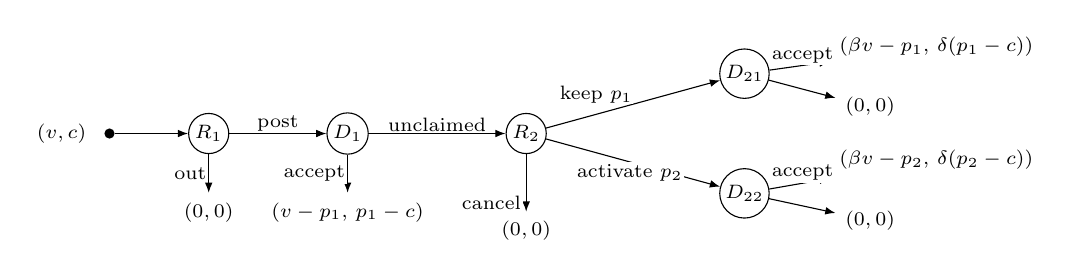
\begin{tikzpicture}[
x=0.84cm,y=0.80cm,
nd/.style={circle,draw,inner sep=1.1pt,minimum size=4.5mm,font=\scriptsize},
term/.style={font=\scriptsize,align=center},
edge/.style={-{Latex[length=1.3mm]},thin},
lab/.style={font=\scriptsize,fill=white,inner sep=0.7pt}
]
\node[circle,fill=black,inner sep=1.3pt] (Nat) at (0,0) {};
\node[left=1mm of Nat,font=\scriptsize] {$(v,c)$};
\node[nd] (R1) at (1.5,0) {$R_1$};
\draw[edge] (Nat) -- (R1);
\node[term] (out) at (1.5,-1.25) {$(0,0)$};
\node[nd] (D1) at (3.6,0) {$D_1$};
\draw[edge] (R1) -- node[lab,left] {out} (out);
\draw[edge] (R1) -- node[lab,above] {post} (D1);
\node[term] (early) at (3.6,-1.25) {$(v-p_1,\,p_1-c)$};
\node[nd] (R2) at (6.3,0) {$R_2$};
\draw[edge] (D1) -- node[lab,left] {accept} (early);
\draw[edge] (D1) -- node[lab,above] {unclaimed} (R2);
\node[term] (ab) at (6.3,-1.55) {$(0,0)$};
\node[nd] (D21) at (9.6,0.95) {$D_{21}$};
\node[nd] (D22) at (9.6,-0.95) {$D_{22}$};
\draw[edge] (R2) -- node[lab,left,pos=.84,xshift=-1pt] {cancel} (ab);
\draw[edge] (R2) -- node[lab,above left,inner sep=0pt] {keep $p_1$} (D21);
\draw[edge] (R2) -- node[lab,below,pos=.48] {activate $p_2$} (D22);
\node[term] (a1) at (12.5,1.38) {$(\beta v-p_1,\,\delta(p_1-c))$};
\node[term] (d1) at (11.5,0.42) {$(0,0)$};
\node[term] (a2) at (12.5,-0.42) {$(\beta v-p_2,\,\delta(p_2-c))$};
\node[term] (d2) at (11.5,-1.38) {$(0,0)$};
\draw[edge] (D21) -- node[lab,above,pos=.55] {accept} (a1);
\draw[edge] (D21) -- (d1);
\draw[edge] (D22) -- node[lab,above,pos=.55] {accept} (a2);
\draw[edge] (D22) -- (d2);
\end{tikzpicture}
\caption{Extensive form.}
\label{fig:game}
\vspace{-5pt}
\end{figure}

For an active menu $0\le p_1<p_2<\beta$, the driver accepts immediately iff
$c\le\ch$.  After rejection, the rider cancels, repeats $p_1$, or activates
$p_2$ according to
\[
v<\frac{p_1}{\beta},\qquad
\frac{p_1}{\beta}\le v\le v^M(\ch),\qquad
v>v^M(\ch),
\qquad
v^M(\ch)=\frac{p_1+p_2-\ch}{\beta}.
\]
The marginal driver's accept-versus-wait indifference gives the WPBE cutoff
\begin{equation}
\ch(p_1,p_2)=\left[p_1-
\frac{\delta(p_2-p_1)(\beta-p_2)}
{\beta(1-p_1)-\delta(\beta-p_2)}\right]_+ ,
\tag{1}
\end{equation}
and equilibrium completion is
\begin{equation}
M_1(p_1,p_2)=(1-p_1)\ch+
\frac{(\beta-p_2)(p_2-\ch)}{\beta}.
\tag{2}
\end{equation}
Thus the cutoff is calculated from the WPBE; the platform then optimizes over
menus subject to this equilibrium response.

Fixing a target cutoff reduces the two-price problem to one dimension.  The
unique continuation envelope and its implementing first price are
\begin{equation}
\widehat p_2(\ch)=\frac{\beta+\ch}{2},\qquad
\widehat p_1(\ch)=
\frac{1+\ch-\sqrt{\Delta(\ch)}}2,\qquad
\Delta(\ch)=(1-\ch)^2-\frac{\delta}{\beta}(\beta-\ch)^2.
\tag{3}
\end{equation}
Substitution into (2) gives
\begin{equation}
M_1^*=\max\left\{\frac14,\ \max_{\ch\in[0,\beta]}J_\delta(\ch)\right\},
\quad
J_\delta(\ch)=
\frac{\ch[1-\ch+\sqrt{\Delta(\ch)}]}2
+\frac{(\beta-\ch)^2}{4\beta}.
\tag{4}
\end{equation}
If $\beta\le1/2$ or $\delta=1$, the optimal value is the flat benchmark
$1/4$.  If $\beta>1/2$ and $\delta<1$, $J_\delta$ is strictly concave and has
a unique interior maximizer, which implements $p_1^*<p_2^*$.

\subsection{Numerical illustration}

At $\beta=\delta=4/5$, the first-order condition becomes
$12-20\ch=5\ch\sqrt{9-10\ch}$.  Squaring yields
$(5\ch-4)(50\ch^2+75\ch-36)=0$; checking the unsquared equation and
feasibility leaves the positive root of the quadratic.  Its discriminant is
$75^2+4(50)(36)=225\cdot57$, which explains the appearance of $\sqrt{57}$:
\[
\ch^*=\frac{3(\sqrt{57}-5)}{20}=.382475,\quad
p_1^*=\frac{11+\sqrt{57}}{40}=.463746,\quad
p_2^*=\frac{1+3\sqrt{57}}{40}=.591238.
\]
The optimal rescue menu completes $25.9581\%$ of requests, compared with
$25.0000\%$ under the best flat price.

\begin{figure}[H]
\centering
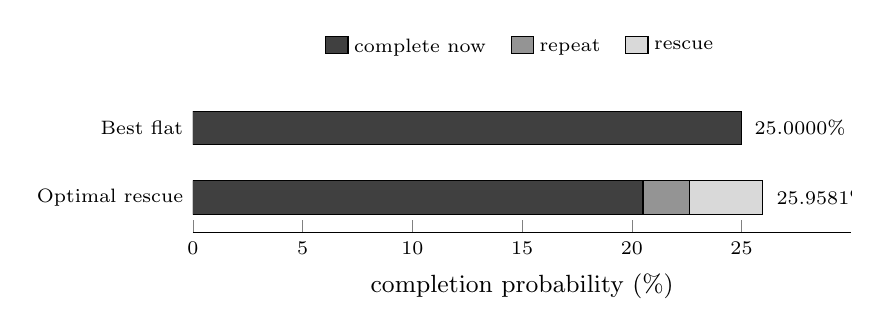
\begin{tikzpicture}
\begin{axis}[
  xbar stacked,
  width=.82\textwidth,
  height=3.35cm,
  xmin=0,xmax=30,
  ymin=-.5,ymax=1.5,
  bar width=12pt,
  xlabel={completion probability (\%)},
  ytick={0,1},
  yticklabels={Optimal rescue,Best flat},
  axis x line*=bottom,
  axis y line*=left,
  y axis line style={draw=none},
  y tick style={draw=none},
  xtick={0,5,10,15,20,25},
  tick label style={font=\scriptsize},
  label style={font=\small},
  legend style={
    at={(0.5,1.18)},anchor=south,draw=none,
    legend columns=3,font=\scriptsize,
    /tikz/every even column/.append style={column sep=7pt}
  }
]
\addplot[fill=black!75,draw=black] coordinates
  {(20.5104,0) (25.0000,1)};
\addlegendentry{complete now}
\addplot[fill=black!42,draw=black] coordinates
  {(2.1208,0) (0,1)};
\addlegendentry{repeat}
\addplot[fill=black!15,draw=black] coordinates
  {(3.3269,0) (0,1)};
\addlegendentry{rescue}
\node[font=\scriptsize,anchor=west] at (axis cs:26.15,0)
  {$25.9581\%$};
\node[font=\scriptsize,anchor=west] at (axis cs:25.15,1)
  {$25.0000\%$};
\end{axis}
\end{tikzpicture}
\caption{Exact-one-driver completion at $\beta=\delta=.8$.  The $0.9581$ pp
gain combines less completion now with repeat and rescue completion later.}
\label{fig:one-driver-numerics}
\end{figure}

\begin{center}
\begin{tabular}{@{}rrrrrr@{}}
\toprule
$\beta$ & $\delta$ & $\ch^*$ & $p_1^*$ & $p_2^*$ & $M_1^*$\\
\midrule
.6 & .5 & .460069 & .467733 & .530034 & .253038\\
.6 & .8 & .478613 & .488210 & .539306 & .251089\\
.8 & .5 & .370421 & .420148 & .585210 & .272458\\
.8 & .8 & .382475 & .463746 & .591238 & .259581\\
.9 & .5 & .329857 & .405843 & .614928 & .286282\\
.9 & .8 & .314018 & .453693 & .607009 & .266932\\
\bottomrule
\end{tabular}
\end{center}
\noindent Each row re-solves the WPBE and optimal menu.  More patient riders
support a larger rescue region; less patient incumbents make waiting less
attractive and increase the completion value of escalation.

\clearpage
\section{From one driver to latent market thickness}

\subsection{Thickness mechanism and prior}

Now only the public mean $m$ is known:
$N^I\sim\operatorname{Pois}(m)$ is latent.  Therefore $m=1$ is not the
publicly known $N=1$ benchmark.  At the same $m$, define
\[
M_R^*(m)=\max_{0\le p_1\le p_2\le1}M_m(p_1,p_2),\qquad
M_F^*(m)=\max_{p\in[0,1]}M_m(p,p),\qquad
V(m)=M_R^*(m)-M_F^*(m).
\]
Here $M_m$ is equilibrium completion.  Thus $100V(m)$ is the percentage-point
gain from allowing the best rescue menu instead of the best flat price in the
\emph{same} market.  It is not the marginal value of adding drivers.

\begin{center}
\begin{tabularx}{\textwidth}{@{}L{2.0cm}XXX@{}}
\toprule
Region & Initial supply & Failure and backup pool & Prior for $V(m)$\\
\midrule
Thin $m$ & Usually no incumbent & Little supply exists to rescue &
Small; first order in $m$\\
Middle $m$ & Initial failure remains material & Failure screens incumbents,
while a useful backup pool often remains & Potentially largest\\
Thick $m$ & Many potential acceptors & Optimized flat pricing already
completes most requests & Small; tends to zero\\
\bottomrule
\end{tabularx}
\end{center}

The middle region contains the trade-off: a larger pool raises terminal
coverage, but the announced $p_2$ also induces more incumbents to wait.  The
direction is therefore an equilibrium-design question rather than a mechanical
coverage comparison.

\subsection{Deterministic numerical evidence}

The reported simulation is deterministic equilibrium optimization, not Monte
Carlo.  For every $m$, the procedure solves the unique cutoff-WPBE for each
candidate menu, reduces the active branch to one scalar cutoff, checks all
stationary points and boundaries, and compares the result with the optimized
flat price.  The baseline is
\[
F=G=U[0,1],\qquad (\alpha,\beta,\delta,\gamma)=(1,.8,.8,0).
\]

\begin{figure}[H]
\centering
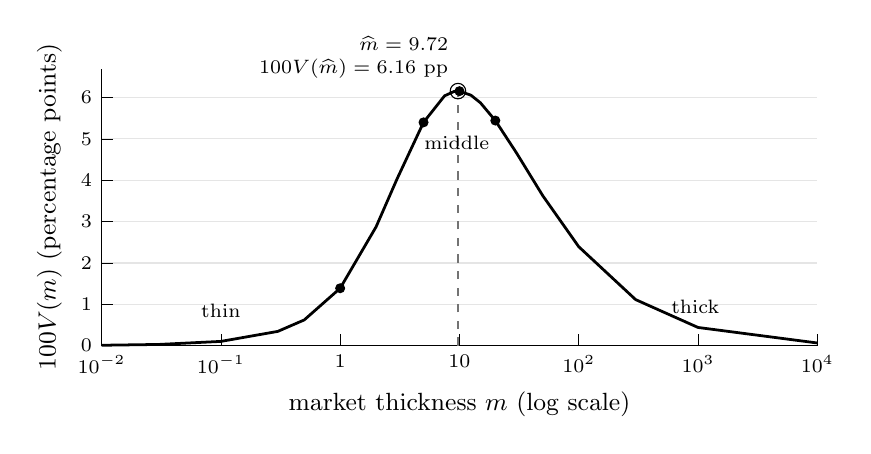
\begin{tikzpicture}
\begin{axis}[
  width=.88\textwidth,
  height=5.1cm,
  xmode=log,
  log basis x=10,
  xmin=.01,xmax=10000,
  ymin=0,ymax=6.7,
  xlabel={market thickness $m$ (log scale)},
  ylabel={$100V(m)$ (percentage points)},
  xtick={.01,.1,1,10,100,1000,10000},
  xticklabels={$10^{-2}$,$10^{-1}$,$1$,$10$,$10^2$,$10^3$,$10^4$},
  ytick={0,1,2,3,4,5,6},
  axis x line*=bottom,
  axis y line*=left,
  axis line style={black,semithick},
  tick style={black},
  tick label style={font=\scriptsize},
  label style={font=\small},
  ymajorgrids=true,
  grid style={black!10},
  clip=false
]
\addplot[black,line width=1pt,mark=none] coordinates {
(.01,.00965650) (.03,.02941466) (.1,.10298843) (.3,.34520582)
(.5,.62236762) (1,1.38833324) (2,2.87273023) (3,4.03321898)
(5,5.40029926) (7.5,6.04105637) (9,6.14663343) (9.5,6.15571941)
(9.718617,6.15658515) (10,6.15523463) (12.5,6.05650260)
(15,5.87342794) (20,5.44368995) (30,4.66713974)
(50,3.62538949) (100,2.39359797) (300,1.11386706)
(1000,.44038496) (10000,.06481155)
};
\addplot[only marks,black,mark=*,mark size=1.6pt] coordinates {
(1,1.38833324) (5,5.40029926) (10,6.15523463) (20,5.44368995)
};
\addplot[only marks,mark=o,mark size=2.8pt,black,fill=white]
coordinates {(9.718617,6.15658515)};
\draw[black!55,dashed,thin]
  (axis cs:9.718617,0) -- (axis cs:9.718617,6.15658515);
\node[anchor=south east,font=\scriptsize,align=right]
  at (axis cs:9.718617,6.24)
  {$\widehat m=9.72$\\$100V(\widehat m)=6.16$ pp};
\node[font=\scriptsize] at (axis cs:.10,.85) {thin};
\node[font=\scriptsize] at (axis cs:9.5,4.9) {middle};
\node[font=\scriptsize] at (axis cs:950,.95) {thick};
\end{axis}
\end{tikzpicture}
\caption{Optimized rescue value across thickness.  Positivity, continuity,
and both endpoint limits are analytical; the connected values and apparent
single hump are numerical.}
\label{fig:Vm}
\end{figure}

\begin{center}
\begin{tabular}{@{}rrrrrrr@{}}
\toprule
$m$ & $\ch^*$ & $p_1^*$ & $p_2^*$ &
$M_R^*$ & $M_F^*$ & $100V(m)$\\
\midrule
1  & .320340 & .391928 & .546378 & .213230 & .199346 & 1.3883 pp\\
5  & .197789 & .236946 & .413098 & .597813 & .543810 & 5.4003 pp\\
10 & .132863 & .155922 & .310306 & .755154 & .693602 & 6.1552 pp\\
20 & .080430 & .092538 & .208054 & .862392 & .807956 & 5.4437 pp\\
\bottomrule
\end{tabular}
\end{center}

The largest value located is at
$(\widehat m,\ch^*,p_1^*,p_2^*)=(9.718617,.135370,.159002,.314745)$.
Across the four highlighted markets, the selected cutoff and both prices fall,
yet rescue coverage rises because the platform draws from a larger pool.

\begin{figure}[H]
\centering
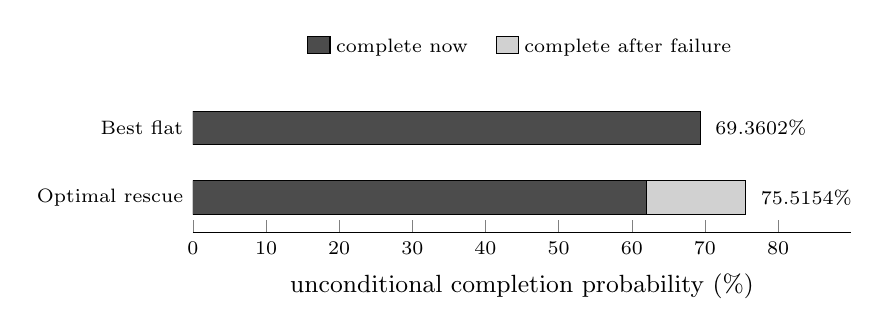
\begin{tikzpicture}
\begin{axis}[
  xbar stacked,
  width=.82\textwidth,
  height=3.35cm,
  xmin=0,xmax=90,
  ymin=-.5,ymax=1.5,
  bar width=12pt,
  xlabel={unconditional completion probability (\%)},
  ytick={0,1},
  yticklabels={Optimal rescue,Best flat},
  axis x line*=bottom,
  axis y line*=left,
  y axis line style={draw=none},
  y tick style={draw=none},
  xtick={0,10,20,30,40,50,60,70,80},
  tick label style={font=\scriptsize},
  label style={font=\small},
  legend style={
    at={(0.5,1.18)},anchor=south,draw=none,
    legend columns=2,font=\scriptsize,
    /tikz/every even column/.append style={column sep=8pt}
  }
]
\addplot[fill=black!70,draw=black] coordinates
  {(62.0532,0) (69.3602,1)};
\addlegendentry{complete now}
\addplot[fill=black!18,draw=black] coordinates
  {(13.4622,0) (0,1)};
\addlegendentry{complete after failure}
\node[font=\scriptsize,anchor=west] at (axis cs:76.3,0) {$75.5154\%$};
\node[font=\scriptsize,anchor=west] at (axis cs:70.1,1) {$69.3602\%$};
\end{axis}
\end{tikzpicture}
\caption{At $m=10$, rescue sacrifices $7.3070$ pp of immediate completion and
recovers $13.4622$ pp after failure, for a net gain of $6.1552$ pp.}
\label{fig:m10-decomposition}
\end{figure}

\begin{figure}[H]
\centering
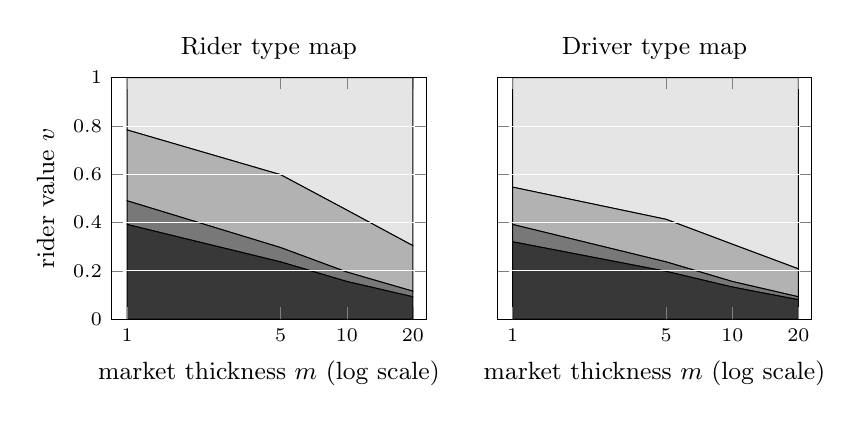
\begin{tikzpicture}
\begin{groupplot}[
  group style={group size=2 by 1,horizontal sep=.9cm},
  width=.46\textwidth,
  height=4.65cm,
  xmode=log,
  log basis x=10,
  xmin=.85,xmax=23,
  ymin=0,ymax=1,
  xtick={1,5,10,20},
  xticklabels={$1$,$5$,$10$,$20$},
  ytick={0,.2,.4,.6,.8,1},
  stack plots=y,
  area style,
  axis on top,
  ymajorgrids,
  grid style={white,line width=.25pt},
  tick label style={font=\scriptsize},
  label style={font=\small},
  title style={font=\small,yshift=-1mm},
  every axis plot/.append style={draw=black,line width=.35pt,mark=none}
]
\nextgroupplot[title={Rider type map},xlabel={market thickness $m$ (log scale)},ylabel={rider value $v$}]
\addplot[fill=black!78] coordinates {(1,.391928) (5,.236946) (10,.155922) (20,.092538)} \closedcycle;
\addplot[fill=black!53] coordinates {(1,.097982) (5,.059237) (10,.038981) (20,.023134)} \closedcycle;
\addplot[fill=black!30] coordinates {(1,.293176) (5,.301516) (10,.256619) (20,.188316)} \closedcycle;
\addplot[fill=black!10] coordinates {(1,.216915) (5,.402301) (10,.548478) (20,.696012)} \closedcycle;
\nextgroupplot[title={Driver type map},xlabel={market thickness $m$ (log scale)},yticklabels=\empty]
\addplot[fill=black!78] coordinates {(1,.320340) (5,.197789) (10,.132863) (20,.080430)} \closedcycle;
\addplot[fill=black!53] coordinates {(1,.071587) (5,.039157) (10,.023059) (20,.012107)} \closedcycle;
\addplot[fill=black!30] coordinates {(1,.154450) (5,.176151) (10,.154384) (20,.115517)} \closedcycle;
\addplot[fill=black!10] coordinates {(1,.453622) (5,.586902) (10,.689694) (20,.791946)} \closedcycle;
\end{groupplot}
\end{tikzpicture}
\vspace{1pt}

{\scriptsize Rider:\quad
\regionkey{black!78}{no post}\quad
\regionkey{black!53}{cancel}\quad
\regionkey{black!30}{repeat $p_1$}\quad
\regionkey{black!10}{rescue $p_2$}\par
Driver:\quad
\regionkey{black!78}{accept now}\quad
\regionkey{black!53}{accept either later}\quad
\regionkey{black!30}{rescue only}\quad
\regionkey{black!10}{never accept}}
\caption{Type regions at $m=1,5,10,20$.  Each vertical slice partitions
$[0,1]$.  Rider rescue mass grows from $.2169$ to $.6960$, while pool-level
rescue coverage rises from $.2023$ to $.9221$.  Type shares are not path
probabilities.}
\label{fig:thickness-regions}
\end{figure}

\clearpage
\section{Formal thickness model}

\subsection{Primitives and timing}

The numerical pattern motivates a model that separates the size and
composition of continuation supply.

\begin{center}
\begin{tabularx}{\textwidth}{@{}L{1.6cm}L{2.0cm}XL{3.0cm}@{}}
\toprule
Param. & Domain & Economic object & Baseline numerics\\
\midrule
$m$ & $(0,\infty)$ & Public mean incumbent supply,
$N^I\sim\operatorname{Pois}(m)$ & varied\\
$\alpha$ & $[0,1]$ & Survival probability of a waiting incumbent & $1$\\
$\gamma$ & $[0,\infty)$ & Fresh-entry intensity,
$N^E\sim\operatorname{Pois}(\gamma m)$ & $0$\\
$\beta$ & $(0,1]$ & Rider discount factor & $.8$\\
$\delta$ & $(0,1]$ & Incumbent discount factor & $.8$\\
$F$ & continuous CDF & Persistent incumbent and entrant cost distribution &
$U[0,1]$\\
$G$ & continuous CDF & Rider value distribution & $U[0,1]$\\
\bottomrule
\end{tabularx}
\end{center}

All primitives and the committed menu are common knowledge; realized counts
and types are latent except to the driver who owns each type.

\begin{enumerate}[label=\textbf{Stage \arabic*.}]
\item \textbf{Commitment.}  The platform observes $m$ and commits to
$0\le p_1\le p_2\le1$; $p_2$ is available only after universal rejection.
\item \textbf{Rider entry.}  The rider observes $v\sim G$ and chooses whether
to post.
\item \textbf{Incumbent response.}  A latent
$N^I\sim\operatorname{Pois}(m)$ pool draws persistent costs $c_i\sim F$.
Drivers simultaneously accept $p_1$ or wait without observing pool size or
rival actions.
\item \textbf{Assignment or public failure.}  One acceptor is selected
uniformly.  Otherwise, universal rejection becomes public but does not reveal
the count or costs.
\item \textbf{Rider continuation.}  The rider cancels, repeats $p_1$, or
activates $p_2$ using $v$, the menu, and the failure posterior.
\item \textbf{Survival, entry, and terminal assignment.}  Each waiting
incumbent survives independently with probability $\alpha$; independently,
$N^E\sim\operatorname{Pois}(\gamma m)$ fresh drivers arrive.  At the active
$p_j$, one acceptor is selected uniformly.  A selected incumbent receives
$\delta(p_j-c_i)$ and a selected entrant receives $p_j-c_i$.
\end{enumerate}

The baseline figures set $\gamma=0$ to isolate strategic waiting.  The formal
extension retains both screened surviving incumbents and unscreened fresh
entrants; they cannot generally be collapsed into a single thickness scalar.

\subsection{Cutoff-WPBE and menu solution}

In an anonymous symmetric pure-cutoff WPBE, incumbents accept $p_1$ iff
$c_i\le\ch$.  A candidate cutoff therefore determines both the failure
posterior and the supply available after failure.  Poisson thinning gives
\[
\phi(x)=\frac{1-e^{-x}}x,\quad \phi(0)=1,\qquad
\lambda_j(\ch)=m\{\alpha[F(p_j)-F(\ch)]+\gamma F(p_j)\},\qquad
C_j(\ch)=1-e^{-\lambda_j(\ch)}.
\]
Here $\phi$ is a focal driver's expected assignment share.  In $\lambda_j$,
$m\alpha[F(p_j)-F(\ch)]$ is the screened mass of surviving incumbents and
$m\gamma F(p_j)$ is the unscreened entrant mass.  Their sum determines
terminal coverage $C_j$.

\paragraph{Rider continuation.}
The rider posts iff $v\ge p_1$.  After universal rejection, she compares
\[
0,\qquad C_1(\ch)(\beta v-p_1),\qquad
C_2(\ch)(\beta v-p_2).
\]
When $C_2(\ch)>C_1(\ch)$, repeat and rescue are equally valuable at
\begin{equation}
v^M(\ch)=
\frac{p_2C_2(\ch)-p_1C_1(\ch)}
{\beta[C_2(\ch)-C_1(\ch)]}.
\tag{5}
\end{equation}
Thus the conditional rider masses are
\[
\eta^{\rm rep}(\ch)=
\Pr\!\left\{\frac{p_1}{\beta}\le v\le v^M(\ch)\,\middle|\,v\ge p_1\right\},
\qquad
\eta^{\rm res}(\ch)=
\Pr\!\left\{v>v^M(\ch)\,\middle|\,v\ge p_1\right\},
\]
with empty regions assigned zero mass.  If $C_2=C_1$, rescue adds no
coverage and is unused.

\paragraph{Driver cutoff.}
Put $\eta^1=\eta^{\rm rep}$ and $\eta^2=\eta^{\rm res}$.  A focal incumbent
of type $c$ compares immediate acceptance with discounted waiting:
\begin{align}
A(c;\ch)&=\phi(mF(\ch))(p_1-c),\nonumber\\
W(c;\ch)&=\delta\alpha e^{-mF(\ch)}
\sum_{j=1}^2\eta^j(\ch)\phi(\lambda_j(\ch))(p_j-c)^+.
\tag{6}
\end{align}
The factors in $W$ are, in order, incumbent discounting, own survival,
universal rejection by rivals, the probability of each rider continuation
action, terminal assignment share, and terminal surplus.  An interior cutoff
solves $A(\ch;\ch)=W(\ch;\ch)$; one-sided inequalities apply at $0$ and
$p_1$.  In the uniform no-entry model this equation has a unique cutoff value
for every menu.

\paragraph{Completion and platform objective.}
Once the cutoff and rider regions have been recovered, completion is
\begin{equation}
M_m(p_1,p_2;\ch)=(1-G(p_1))
\left[1-e^{-mF(\ch)}+e^{-mF(\ch)}
\{\eta^{\rm rep}C_1+\eta^{\rm res}C_2\}\right].
\tag{7}
\end{equation}
The terms are posting, first-window completion, and failure followed by
terminal completion.  The platform maximizes (7) only after imposing
(5)--(6); this is the WPBE-constrained menu-design problem.

For $F=G=U[0,1]$ and $\gamma=0$, put $k=\alpha m$ and
\[
S_m(\ch,p_2)=(\beta-p_2)\{1-e^{-k(p_2-\ch)}\},\qquad
h_m(\ch)=\frac{e^{m\ch}-1}{\ch},\quad h_m(0)=m.
\]
The active branch admits an exact three-step reduction:
\begin{enumerate}[label=\textbf{\arabic*.},leftmargin=1.0cm]
\item \textbf{Given $\ch$, solve $p_2$.}
Rider switching makes continuation completion telescope to
$S_m(\ch,p_2)/\beta$.  Its unique maximizer solves
\[
e^{k(\widehat p_2-\ch)}-1=k(\beta-\widehat p_2),\qquad
\widehat p_2=
\beta-\frac{W_0(e^{1+k(\beta-\ch)})-1}{k}.
\]
\item \textbf{Use driver indifference to solve $p_1$.}
With $p_2=\widehat p_2$, equation (6) becomes
\[
(1-p_1)(p_1-\ch)
=\frac{\delta S_m(\ch,\widehat p_2)}{\beta h_m(\ch)}.
\]
The root satisfying $\ch\le p_1\le\widehat p_2$ is
\[
\widehat p_1^\delta=
\frac{1+\ch-
\sqrt{(1-\ch)^2-\dfrac{4\delta S_m(\ch,\widehat p_2)}
{\beta h_m(\ch)}}}{2}.
\]
\item \textbf{Optimize the remaining cutoff.}
Substitution into (7) leaves
\[
J_{\delta,m}(\ch)=
[1-\widehat p_1^\delta](1-e^{-m\ch})
+e^{-m\ch}\frac{S_m(\ch,\widehat p_2)}{\beta},
\qquad \ch\in[0,\beta].
\]
\end{enumerate}
Consequently,
\[
\ch^*(m)\in\arg\max_{\ch\in[0,\beta]}J_{\delta,m}(\ch),\qquad
p_1^*(m)=\widehat p_1^\delta(\ch^*(m);m),\qquad
p_2^*(m)=\widehat p_2(\ch^*(m);m).
\]
Thus both prices are obtained from the WPBE, not from an unconstrained price
grid.  The optimized flat benchmark has
\[
p_F^*(m)=\frac{1+m-W_0(e^{1+m})}{m}.
\]

\section{Evidence boundary, extensions, and literature}

\subsection{Established results and conjectures}

\begin{center}
\begin{tabularx}{\textwidth}{@{}L{2.3cm}X@{}}
\toprule
Status & Statement\\
\midrule
Established & In the uniform no-entry model, every menu has a unique cutoff
value in the maintained WPBE class and the optimal menu reduces to the scalar
problem above.  For $\beta\ge1/2$,
$V(m)>0$ at every finite $m$, $V$ is continuous, and
$V(m)\to0$ as $m\downarrow0$ and $m\to\infty$.  Hence at least one positive
finite maximizer exists.\\
Established limits & With $\alpha=1$, $\gamma=0$, and
$\beta=\delta=.8$,
\[
\lim_{m\downarrow0}\frac{V(m)}m
=M_1^*-\frac14
=\frac{461-57\sqrt{57}}{3200}=.00958107.
\]
Thus the exact-one-driver gain is the thin-market coefficient.  For fixed
positive $\alpha,\beta$ and $\gamma=0$, $V(m)\sim(\log m)/m$ in thick
markets.\\
Numerical evidence & The baseline curve has one located peak
$\widehat m=9.718617$ with a $6.1566$ pp gain.  At
$m=1,5,10,20$, the selected $\ch^*,p_1^*,p_2^*$ fall, while rider rescue mass
and pool-level rescue coverage rise.\\
Conjectures & For $\beta\ge1/2$ in the uniform no-entry model, $V(m)$ may be
strictly single-peaked with a unique maximizer.  A monotone selection of
$\ch^*(m),p_1^*(m),p_2^*(m)$ may also exist, but neither optimizer uniqueness
nor global monotonicity is proved.  For $\beta<1/2$, an initial zero plateau
already rules out strict single-peakedness in this form.\\
Mixed supply & With $\alpha<1$ and $\gamma>0$, a small rescue increment
strictly improves an optimized flat policy under an explicit rider-activity
condition; when the condition fails strictly, the increment is unused.
Holding continuation headcount or price-marginal capacity fixed, a larger
incumbent share locally intensifies cutoff erosion.  Global menu design and
the full shape of $V_{\alpha,\gamma}(m)$ remain open; composition effects on
completion can be nonmonotone.\\
\bottomrule
\end{tabularx}
\end{center}

\clearpage
\subsection{Position relative to the closest literature}

\begin{center}
\begin{tabularx}{\textwidth}{@{}L{3.6cm}L{4.3cm}>{\raggedright\arraybackslash}X@{}}
\toprule
Literature & Existing mechanism & Additional object here\\
\midrule
\citet{LiKuo2013} & Dutch clock with uncertain bidder count &
Private rider continuation and completion design\\
\citet{Chen2012}; \citet{CorreaEtAl2016} &
Strategic waiting and contingent preannouncement &
Drivers wait for higher pay under assignment competition\\
\citet{HuHuZhu2022} & Two-sided temporal response to surge pricing &
Same-request failure-contingent commitment and posterior updating\\
\citet{LeeLi2023} & Screened incumbents and later entrants in search &
Posted payments with abandon, repeat, and rescue\\
\citet{LoertscherMuirTaylor2022} & Optimal accumulation of market thickness &
Value of rescue pricing while holding the same $m$ fixed\\
\bottomrule
\end{tabularx}
\end{center}

\noindent The contribution is not two prices, Poisson supply, or strategic
waiting separately.  It is their joint cutoff-WPBE design with latent realized
competition, universal-rejection learning, private rider continuation,
screened incumbents, unscreened entrants, and a completion objective.

\paragraph{Empirical calibration placeholder.}
A request-level calibration needs the announced $(p_1,p_2)$, a public
pre-window thickness proxy, initial exposures and universal rejection, rider
continuation, driver identities linking survivors to the first window, fresh
entrant exposure, and final completion.  These fields identify or discipline
$(m,\alpha,\gamma,F,G)$ and the dynamic responses governed by
$(\beta,\delta)$.  The paper specifies this mapping but does not insert
synthetic estimates as empirical findings.

\renewcommand{\bibsection}{\paragraph{References.}}
\begin{multicols}{2}
\scriptsize
\raggedcolumns
\interlinepenalty=10000
\setlength{\bibsep}{0pt}
\begin{thebibliography}{99}
\bibitem[Chen(2012)]{Chen2012} Chen, C.-H. 2012. Name your own price at
Priceline.com: Strategic bidding and lockout periods. \emph{Review of Economic
Studies} 79(4), 1341--1369.
\bibitem[Correa et~al.(2016)]{CorreaEtAl2016} Correa, J., R. Montoya,
C. Thraves. 2016. Contingent preannounced pricing policies with strategic
consumers. \emph{Operations Research} 64(1), 251--272.
\bibitem[Hu et~al.(2022)]{HuHuZhu2022} Hu, B., M. Hu, H. Zhu. 2022. Surge
pricing and two-sided temporal responses in ride hailing. \emph{M\&SOM}
24(1), 91--109.
\bibitem[Lee and Li(2023)]{LeeLi2023} Lee, J., D. Li. 2023. Seller compound
search for bidders. \emph{Journal of Industrial Economics} 71(4), 1004--1037.
\bibitem[Li and Kuo(2013)]{LiKuo2013} Li, Z., C.-C. Kuo. 2013. Design of
discrete Dutch auctions with an uncertain number of bidders. \emph{Annals of
Operations Research} 211, 255--272.
\bibitem[Loertscher et~al.(2022)]{LoertscherMuirTaylor2022} Loertscher, S.,
E. Muir, P. G. Taylor. 2022. Optimal market thickness. \emph{Journal of
Economic Theory} 200, 105383.
\end{thebibliography}
\end{multicols}

\end{document}
